\documentclass[journal, a4paper]{IEEEtran}

% some very useful LaTeX packages include:
\usepackage{cite}
\usepackage{plain}
\usepackage{cancel}



%\renewcommand{\citedash}{--}    
%\usepackage{cite}      % Written by Donald Arseneau
                        % V1.6 and later of IEEEtran pre-defines the format
                        % of the cite.sty package \cite{} output to follow
                        % that of IEEE. Loading the cite package will
                        % result in citation numbers being automatically11
                        % sorted and properly "ranged". i.e.,
                        % [1], [9], [2], [7], [5], [6]
                        % (without using cite.sty)
                        % will become:
                        % [1], [2], [5]--[7], [9] (using cite.sty)
                        % cite.sty's \cite will automatically add leading
                        % space, if needed. Use cite.sty's noadjust option
                        % (cite.sty V3.8 and later) if you want to turn this
                        % off. cite.sty is already installed on most LaTeX
                        % systems. The latest version can be obtained at:
                        % http://www.ctan.org/tex-archive/macros/latex/contrib/supported/cite/

\usepackage{graphicx}   % Written by David Carlisle and Sebastian Rahtz
                        % Required if you want graphics, photos, etc.
                        % graphicx.sty is already installed on most LaTeX
                        % systems. The latest version and documentation can
                        % be obtained at:
                        % http://www.ctan.org/tex-archive/macros/latex/required/graphics/
                        % Another good source of documentation is "Using
                        % Imported Graphics in LaTeX2e" by Keith Reckdahl
                        % which can be found as esplatex.ps and epslatex.pdf
                        % at: http://www.ctan.org/tex-archive/info/

%\usepackage{psfrag}    % Written by Craig Barratt, Michael C. Grant,
                        % and David Carlisle
                        % This package allows you to substitute LaTeX
                        % commands for text in imported EPS graphic files.
                        % In this way, LaTeX symbols can be placed into
                        % graphics that have been generated by other
                        % applications. You must use latex->dvips->ps2pdf
                        % workflow (not direct pdf output from pdflatex) if
                        % you wish to use this capability because it works
                        % via some PostScript tricks. Alternatively, the
                        % graphics could be processed as separate files via
                        % psfrag and dvips, then converted to PDF for
                        % inclusion in the main file which uses pdflatex.
                        % Docs are in "The PSfrag System" by Michael C. Grant
                        % and David Carlisle. There is also some information
                        % about using psfrag in "Using Imported Graphics in
                        % LaTeX2e" by Keith Reckdahl which documents the
                        % graphicx package (see above). The psfrag package
                        % and documentation can be obtained at:
                        % http://www.ctan.org/tex-archive/macros/latex/contrib/supported/psfrag/

%\usepackage{subfigure} % Written by Steven Douglas Cochran
                        % This package makes it easy to put subfigures
                        % in your figures. i.e., "figure 1a and 1b"
                        % Docs are in "Using Imported Graphics in LaTeX2e"
                        % by Keith Reckdahl which also documents the graphicx
                        % package (see above). subfigure.sty is already
                        % installed on most LaTeX systems. The latest version
                        % and documentation can be obtained at:
                        % http://www.ctan.org/tex-archive/macros/latex/contrib/supported/subfigure/

\usepackage{url}        % Written by Donald Arseneau
                        % Provides better support for handling and breaking
                        % URLs. url.sty is already installed on most LaTeX
                        % systems. The latest version can be obtained at:
                        % http://www.ctan.org/tex-archive/macros/latex/contrib/other/misc/
                        % Read the url.sty source comments for usage information.

%\usepackage{stfloats}  % Written by Sigitas Tolusis
                        % Gives LaTeX2e the ability to do double column
                        % floats at the bottom of the page as well as the top.
                        % (e.g., "\begin{figure*}[!b]" is not normally
                        % possible in LaTeX2e). This is an invasive package
                        % which rewrites many portions of the LaTeX2e output
                        % routines. It may not work with other packages that
                        % modify the LaTeX2e output routine and/or with other
                        % versions of LaTeX. The latest version and
                        % documentation can be obtained at:
                        % http://www.ctan.org/tex-archive/macros/latex/contrib/supported/sttools/
                        % Documentation is contained in the stfloats.sty
                        % comments as well as in the presfull.pdf file.
                        % Do not use the stfloats baselinefloat ability as
                        % IEEE does not allow \baselineskip to stretch.
                        % Authors submitting work to the IEEE should note
                        % that IEEE rarely uses double column equations and
                        % that authors should try to avoid such use.
                        % Do not be tempted to use the cuted.sty or
                        % midfloat.sty package (by the same author) as IEEE
                        % does not format its papers in such ways.

\usepackage{amsmath}    % From the American Mathematical Society
                        % A popular package that provides many helpful commands
                        % for dealing with mathematics. Note that the AMSmath
                        % package sets \interdisplaylinepenalty to 10000 thus
                        % preventing page breaks from occurring within multiline
                        % equations. Use:
%\interdisplaylinepenalty=2500
                        % after loading amsmath to restore such page breaks
                        % as IEEEtran.cls normally does. amsmath.sty is already
                        % installed on most LaTeX systems. The latest version
                        % and documentation can be obtained at:
                        % http://www.ctan.org/tex-archive/macros/latex/required/amslatex/math/



% Other popular packages for formatting tables and equations include:

%\usepackage{array}
% Frank Mittelbach's and David Carlisle's array.sty which improves the
% LaTeX2e array and tabular environments to provide better appearances and
% additional user controls. array.sty is already installed on most systems.
% The latest version and documentation can be obtained at:
% http://www.ctan.org/tex-archive/macros/latex/required/tools/

% V1.6 of IEEEtran contains the IEEEeqnarray family of commands that can
% be used to generate multiline equations as well as matrices, tables, etc.

% Also of notable interest:
% Scott Pakin's eqparbox package for creating (automatically sized) equal
% width boxes. Available:
% http://www.ctan.org/tex-archive/macros/latex/contrib/supported/eqparbox/

% *** Do not adjust lengths that control margins, column widths, etc. ***
% *** Do not use packages that alter fonts (such as pslatex).         ***
% There should be no need to do such things with IEEEtran.cls V1.6 and later.

\usepackage{booktabs}
\usepackage{xcolor}
\usepackage{array}
\usepackage{caption}
\usepackage{arydshln}
\usepackage{amsfonts}

\def\one{\mathbf{1}}

\setlength{\dashlinedash}{.4pt}
\setlength{\dashlinegap}{.8pt}

\newcommand{\ct}[1]{\multicolumn{1}{c}{#1}}

\def\vsep{\vspace{3mm}\\}

\newcommand{\rpm}{\sbox0{$1$}\sbox2{$\scriptstyle\pm$}
	\raise\dimexpr(\ht0-\ht2)/2\relax\box2 } % plus ou moins
\newcommand{\h}[1]{\colorbox{yellow}{#1}}

% Your document starts here!
\usepackage{Sweave}
\begin{document}

% Define document title and author
\title{\Large{Identifying Relevant Genes Related Atopic Dermatitis  to  using Transcriptomic}}
\author{%
\begin{tabular}{c} Creel, Kristin \\ ISPED \\ University of Bordeaux \\ \texttt{kristin.creel@etu.u-bordeaux.fr} \end{tabular} \and
\begin{tabular}{c} Dong, Larry \\ Department of Epidemiology, Biostatistics \\ and Occupational Health \\ McGill University \\ \texttt{larry.dong@mail.mcgill.ca} \end{tabular} \and
\begin{tabular}{c} Nama Ravi, Sneha Keerthi \\ ISPED \\ University of Bordeaux \\ \texttt{sneha-keerthi.nama-ravi@etu.u-bordeaux.fr} \end{tabular}}
\maketitle

% Write abstract here


\Sconcordance{concordance:version-1.tex:version-1.Rnw:%
1 155 1 1 0 211 1}


\section*{\textbf{Abstract}}

\textbf{Background --- } Atopic dermatitis (AD), a skin disease mainly characterized by the inflammation of the skin, affects $15-20 \%$ children and $1-3\%$ adults worldwide. While some literature regarding its causes and its pathogenesis are available, further investigation regarding the transcriptomic expression of AD samples could lead to new findings.%little research has been conducted at the transcriptomic level of this illness.

\textbf{Methods ---} Transcriptomic data for lesional and non-lesional samples was provided by the MAARS study, a cohort study whose goal is to better understand skin diseases due to allergies and autoimmune disorders. Exploratory data analysis using principle component analysis (PCA) was first performed in the attempt to visualize the separability of the AD samples from the controls. Two data-driven methods in investigating the genes prone to be associated with AD were then used in this study: differential gene expression (DGE) analysis in a multiple testing framework and sparse partial least squares (sPLS).

\textbf{Results ---} A total of 81 genes were found to be significantly differentially expressed between lesional and non-lesional skin samples using DGE, whereas 42 were obtained from sPLS. In these sets of identified genes, 7 were found to be common to both sets: KRT16, PRSS27, S100A9, S100A12, PI3, GJB2, ARK1B10.

\textbf{Conclusion ---} The 7 identified genes were found to be linked to inflammatory processes, lipid metabolism and skin barrier pathways. However, potential confounding in the results due to race, patient age and allergies will further investigation. 

\textbf{Keywords:} Atopic dermatitis, transcriptomics, gene annotation, differential gene expression, sparse partial least squares.

\section{\textbf{Introduction}}

Atopic dermatitis (AD) or atopic eczema is an itchy, inflammatory skin condition characterised by poorly defined erythema with edema vesicles, and weeping in the acute stage and lichenification in the chronic stage. The global prevalence is $15-20 \%$ in children and $1-3\%$ in adults, posing a significant burden on health-care resources and patients’ quality of life \cite{nutten2015atopic}. The etiological factors associated with the initiation and progress of the disease are known to be genetic, environmental and immunological that affects the epithelial barrier-immunity interplay \cite{peng2015pathogenesis}.\\

Clinical investigations and discoveries in molecular medicine have positively identified $46$ genes linked to AD. Mutations in filaggrin (FLG) genes (influencing intermediate filament protein filaggrin expression) are most common in the AD diseased population, it affects $10-50\%$ of AD patients worldwide. Few additional barrier genes encoded by the epidermal differentiation complex (EDC) locus chromosome 1q21, including claudins, loricrin (LOR), involucrin (IVL), SPINK5, AND tmem79/matt, are also associated with AD. The genes of innate immune system such as NOD1, NOD2, TLR2, CD14, and DEFB1, all of which encode the integral factors in cutaneous immunologic response to non-specific antigens may also experience mutations and cause AD \cite{guttman2017atopic}. Studies have identified FLG gene mutation to be the most significant risk factor for AD, followed by the genes in the type 2 T helper lymphocyte (Th2) signalling pathways. Additionally, gene profiling assays demonstrated AD is associated with decreased gene expression of epidermal differentiation complex genes and elevated Th2 and Th17 genes. Hypomethylation of TSLP and FCER1G in AD were also reported; and miR-155, which targets the immune suppressor CTLA-4, was found to be significantly over-expressed in infiltrating T cells in AD skin lesions \cite{guttman2017atopic, bin2016genetic}.\\

This study attempts to examine the degree of dissimilarity between the transcriptomic expression between lesional and non-lesional samples in participants with atopic dermatitis. Data-driven methods are employed to identify relevant genes that are related to a flare-up in better understanding the molecular mechanisms.

\section{\textbf{Materials and Methods}}

\subsection{\textbf{Data Source}}

The data at hand comes from the Microbes in Allergy and Autoimmunity Related to the Skin (MAARS). The purpose of this multidisciplinary research consortium is to better understand the characteristics surrounding two major chronic inflammatory skin diseases: atopic dermatitis and psoriasis\cite{MAARS}. In the MAARS study, these two illnesses are investigated from different scientific perspectives and one of the research directions involved exploring the transcriptomic data of lesional and non-lesional samples in patients with atopic dermatitis, psoriasis (PSO) and neither of the two studied skin diseases.\\

% the relationship between the host and its microbiome 

\subsubsection*{\textbf{Data Management}}

Demographic data for all patients were available alongside their known allergies, concomitant medication and transcriptomic data for sequenced samples. A total of $1317$ patients with AD, PSO or neither illness were examined and $618$ samples were sequenced. However, because it was only of interest to assess RNA expression levels in samples from patients with atopic dermatitis, two sets of data were discarded prior to conducting subsequent analyses: participants with AD who have no sequenced samples and genetic information for samples from healthy individuals and those with psoriasis. The normalization procedure for transcriptomic data was already performed prior to obtaining the data for this anlysis. No genetic information was missing, so statistical methods for imputation were not needed for this study.


\subsection{\textbf{Exploratory Data Analysis}}

Exploratory data analysis was conducted to better understand the data at hand from a data-driven perspective. To this end, an MA diagram was plotted alongside several clustering methods which were used to help depict possible underlying patterns from the MAARS transcriptomic data: principal component analysis (PCA) and hierarchical clustering \cite{maaten2008visualizing, friedman2001elements}. In statistical machine learning, clustering techniques falls under unsupervised learning, which is a paradigm that attempts to perform inference on data without response variables or ``labels" \cite{friedman2001elements}. Here, the sample labels are the lesional status of the skin sample and the primary purpose of performing such unsupervised analyses was to visually assess the separability of the samples using their transcriptomic information.

\subsection{\textbf{Statistical Analysis}}

%\subsubsection{Differential Gene Expression Analysis}

The overarching goal of the statistical analysis was to determine the relevant genes from a transcriptomic datatset that are associated to AD. The analysis plan was performed two-fold; the identification of genes highly associated with AD was first performed using differential gene expression analysis (DGE) within a multiple hypothesis testing framework. The transcriptomic data was available as a continuous variable since the microarray data has been normalized. Secondly, an analysis using sparse partial least squares (sPLS) was conducted to identify genes that can ``best explain" the variability in the lesional status of the sequenced samples. Information regarding the ten first components were retained and a different number of genes was selected for each constructed component; the number of variables selected was determined using a 10-fold cross-validation method.\\

Let $Y_{ij} \in \mathbb{R}$ denote the gene expression level of gene $j$ in sample $i$ and let $X_i \in \{0, 1\}$ represent its lesional status. Because multiple samples can come from a same individual, confounding bias caused by intersample correlation could have occured if not taken into account. Let $\mathcal{P}$ denote the set of all patients and $pat(i) \in \mathcal{P}$ is used to represent the patient to which belongs sample $i$. The following linear model was fitted:
\begin{align*}
  Y_{ij} &=\beta_{0j} + \beta_{1j}X_i + \beta_{pat(i)}\one_{pat(i)} + \epsilon_{ij}
\end{align*}
% By construction, $\one_{pat(i) = k} = 1$ for exactly one $k \in \mathcal{P}$ and $\big\vert \mathcal{P}\big\vert < n$.\\

\noindent where the coefficient $\beta_{pat(i)}$ accounts for the intersample correlation for samples which are obtained from the same patient. Originally developped for two-color microarray experiments, it is now commonplace to use an empirical Bayes method to analyze differential gene expression with linear models like the one above \cite{smyth2004linear}. In a hypothesis framework, the following distributional assumptions for $\beta_{1j}$ are assumed for all genes $j$:
\begin{align*}
  H_0:\qquad \beta_{1j} \,\big\vert\, \sigma^2_j &\sim \mathcal{N}\left(0, \sigma^2_j\right)\\
  H_1:\qquad \beta_{1j} \,\big\vert\, \sigma^2_j &\,\,\cancel{\sim}\,\, \mathcal{N}\left(0, \sigma^2_j\right)
\end{align*}

\noindent where the $p$-values were obtained using the rank of each gene's $t$-statistics as described by G. Smyth (2004) and they were adjusted using the Benjamini-Hochberg procedure to reduce the error in false discovery rate prone to be inflated due to performing multiple parallel statistical tests \cite{smyth2004linear, benjamini2010discovering}. A significance level of $0.05$ was used in determining the genes highly associated with the outcome of interest, the lesional status of sequenced samples; an MA plot was used to visually quantify the amount of potentially significant genes.\\

%An ensemble learning prediction model was then implemented to assess predictability of sample lesional status; this binary model was chosen due to its strengths in obtaining better predictions as it weights multiple models according to how well each perform on this specific task\cite{friedman2001elements}. MENTION VARIABLE SELECTION. The receiving operating characteristic (ROC) curve is often used to evaluate data-driven binary prediction models and the area under this curve (AUROC) was used here to quantify the goodness of the prediction model\cite{hanley1982meaning}. Internal validation was performed conducted via bootstrap resampling whereby a thousand samples of the data were sampled without replacement to create an empirical $95\%$ confidence interval for the overall AUROC\cite{efron1994introduction}.%using leave-one-out cross-validation method whereby the AUROC was evaluated at every iteration\cite{efron1994introduction}. %An additional sensitivity analysis of the prediction model was

%This goodness of fit metric was used on ensemble learning model \cite{efron1994introduction}\\

\section{\textbf{Results}}

In Fig. \ref{fig:pca}, a simple 2D visualization of the results obtained from PCA is available, whereby lesional samples are displayed in black and non-lesional samples are displayed in red.

\begin{figure}[!htp]
    \begin{center}
    \begin{minipage}{0.5 \textwidth}
      \centering
      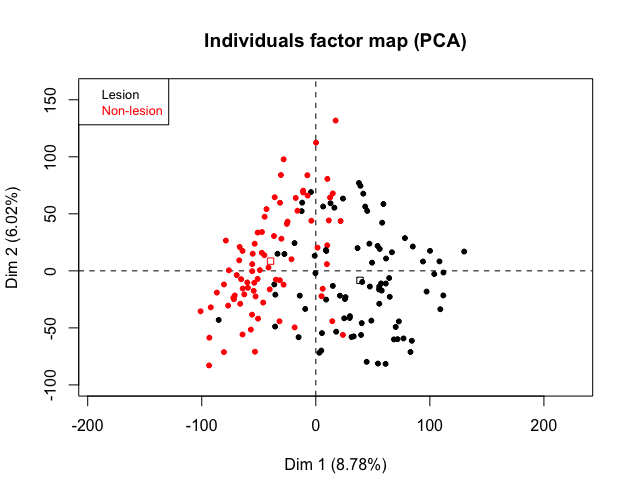
\includegraphics[width=\textwidth]{../exploratory-data-analysis/pca-plot.png}
      \caption{2D representation of samples using the two first principle components obtained by PCA.}
      \label{fig:pca}
    \end{minipage}
  \end{center}
\end{figure}


The horizontal axis represents the first principle component (PC) obtained through PCA and the vertical axis the second; they respectively explain $8.78\%$ and $6.02\%$ of the variance in the transcriptomic data. The Scree plot available in Fig. \ref{fig:scree-plot} is another method of visualizing the amount of variation explained in each constructed PC. While the one of the primary purposes of this plot would help determine the moderate number of PC dimensions needed to explain the a majority of the variation, this plot can also illustrate the decreasing trend of explained variance across constructed PCs.\\%, the scree plot would have a steep curve, followed by a sharp bend, and then a line that straightens out.\\

\begin{figure}[!htp]
    \begin{center}
    \begin{minipage}{0.5 \textwidth}
      \centering
      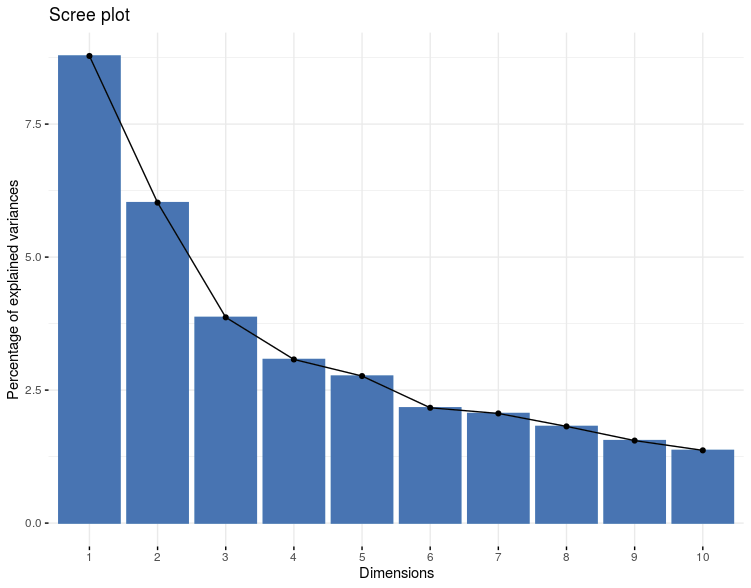
\includegraphics[width=\textwidth]{scree-plot.png}
      \caption{Percentage of variation explained by the first 10 principle components obtained by PCA.}
      \label{fig:scree-plot}
    \end{minipage}
  \end{center}
\end{figure}

A Differential Gene Analysis (DGE) was conducted using a linear model for paired data. The results indicated $81$ genes that differed significantly between the lesioned and non-lesioned skin samples: $65$ that are up-regulated and $16$ that down-regulated.\\% A heatmap illustrating the normalized gene expression levels is displayed below.

A MA plot disaplyed in \ref{fig:MA} was used to visually represent the genes and determine which are up- and down-regulated. In the plot, each dot represents a gene. The x-axis is the average expression of the gene over the mean of normalized counts; the y-axis is the log2 fold change between the lesional statuses. The MA plot below indicates some genes that are up-regulated and fewer that are down-regulated.\\

\begin{figure}[!htp]
  \begin{center}
    \begin{minipage}{0.5 \textwidth}
      \centering
      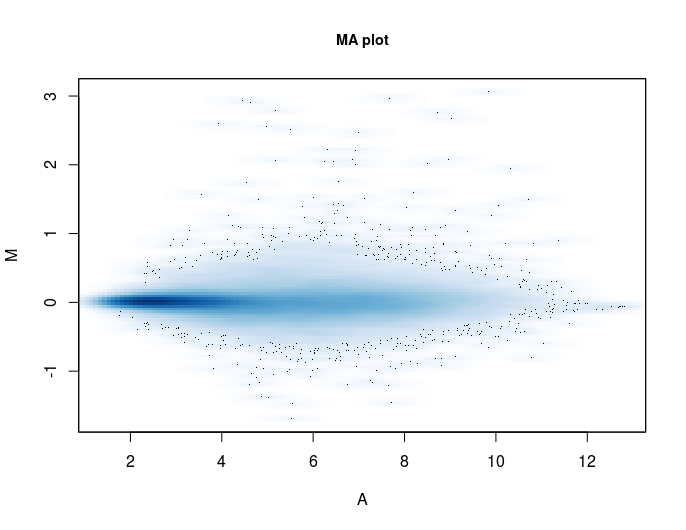
\includegraphics[width=\textwidth]{../analysis/MA-plot-AD-paired-design.png}
      \caption{MA plot for visualization of upregulated and downregulated genes.}
      \label{fig:MA}
    \end{minipage}\\
    \begin{minipage}{0.5 \textwidth}
      \centering
      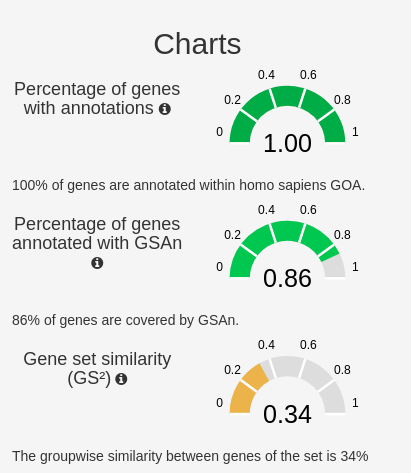
\includegraphics[width=0.75\textwidth]{gsan-charts.png}
      \caption{Descriptive statistics of results obtained with GSAn on the 7 genes of interest.}
      \label{fig:gsan-chart}
    \end{minipage}\\
    \begin{minipage}{0.5 \textwidth}
      \centering
      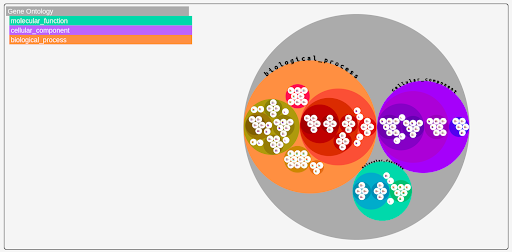
\includegraphics[width=\textwidth]{gene-ontology.png}
      \caption{Diagram showing the groupings of genetic information in the identified genes into three overarching categories: biological processes, cellular components and molecular functions.}
      \label{fig:gene-ontology}
    \end{minipage}
  \end{center}
\end{figure}

\begin{figure*} %occupies two columns
  \centering
  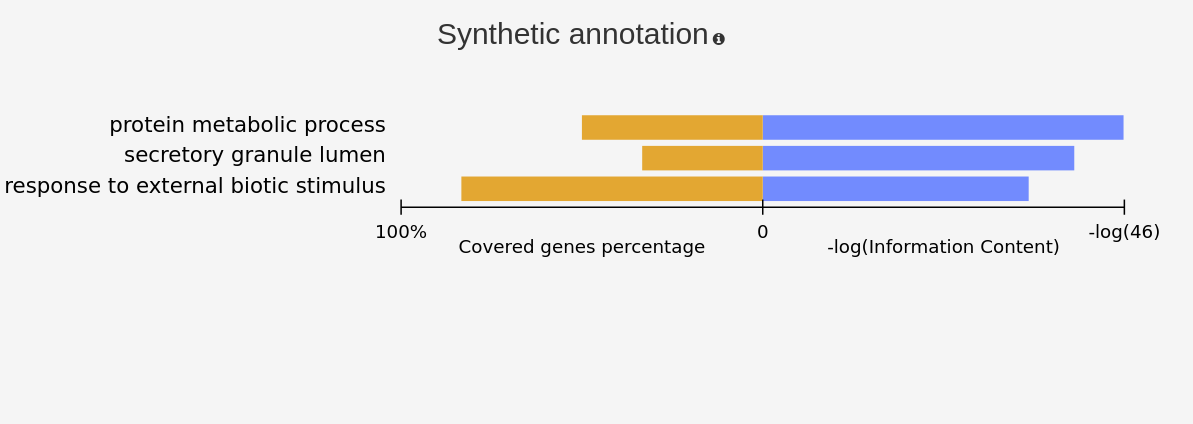
\includegraphics[width=0.85\textwidth]{synthetic-annotation.png}
  \caption{Summary statistics of information and role of the genes of interest.}
  \label{fig:synthetic-annotation}
\end{figure*}


The analysis using sPLS resulted in the identification of 42 genes, 7 of which were found to be common in the two conducted analyses: DGE and sPLS. Genes KRT16, PRSS27, S100A9, S100A12, PI3, GJB2, ARK1B10 were found common in both analyses. Gene annotations using GSAn (Gene Set Annotation) CITATION, which includes a search on the Gene Ontology Database (GOA) as well, were performed for the seven genes that were identified as significant in both the DGE and the sPLS analyses. Using both the gene identifiers and their synonyms, GSAn retained 19 terms, covering 13 out of 16 genes and 6 of them are synthetic terms.\\

Figure \ref{fig:gsan-chart} provides information about the annotated genes within (GOA), the genes covered by GSAn, and the group-wise similarity between them. The first gauge shows excellent gene coverage of $100\%$ within the GOA file. The second gauge shows that $81\%$ of the genes were covered with the GSAn analysis. The third gauge shows that $44\%$ of the genes share a term in both datasets.\\


Figure \ref{fig:gene-ontology} provides more detailed information about the representative terms. Further exploration of the tree will provide additional information on the terms sharing the same informative ancestor or the genes annotated by more than one term. Using this information, information can be obtained on the biological role of these genes in the occurrence of lesional AD.\\

Figure \ref{fig:synthetic-annotation} displays the information content and the gene coverage of the synthetic terms. Functional annotation categories from lesional AD samples include serine endopeptidase activity, protein metabolic process, antimicrobial humoral response, cytoskeleton and toll-like receptor binding.\\

%The results between the DGE and sPLS analysis were compared and seven genes were found to be common in both analyses.  


\section{\textbf{Discussion}}

Differential gene expression analysis helped understand the patterns of expressed genes in the diseased samples which can be used as biomarkers to differentiate them from the control samples. The current analysis considered all atopic dermatitis samples and compared lesional and non-lesional subtypes from the same patients. The current analysis was able to detect much variation in transcriptomic expression between lesional and non-lesional AD skin samples: up to $25\%$ of the variation in the transcriptomic data can be explained by five principal components. However, as displayed in \ref{fig:pca}, PCA demonstrates that the genetic data at hand warrants further investagation as lesional and non-lesional samples visually appears to form two separate groups. Moreoever, in PCA, aach eigenvector defines a principal component and their corresponding eigenvalue is proportional to its explained variance. The eigenvectors with large eigenvalues are the ones that exhibits the most information; the two first components explain $14.8\%$ of the variance in the transcriptomic data.\\%lesional state does not account for much of the differences in the samples.\\

%Unsupervised analysis like PCA and Dendrogram	were used for data exploration. Principal Components Analysis (PCA) is a statistical technique used to explore data during microarray analysis. It is performed to reduce the dimensionality of data by transforming the correlated variables into a smaller number of uncorrelated variables called components. PCA can determine the key variables in the data that best explain the differences in the observations. The matrix of the data used shows rows as samples (individuals) and columns as genes (variables). Each eigenvector defines a principal component and their corresponding eigenvalue is proportional to its explained variance. It is the variance of the component over all the genes. The eigenvectors with large eigenvalues are the ones that exhibits the most information. In our study PC1 and PC2 have an eigenvalue of approximately 2856 and 1965 and it contains the highest variance and information about the genes.\\

The set of seven genes that were identified in both the DGE and sPLS processes were used for gene annotation. The functional annotation of these seven genes shows their roles in inflammatory process (S100A9/A12), lipid metabolism (AKR1B10, AKR1B11) and skin barrier pathways (KRT16 , PRSS27, GJB2, PI3).

\begin{itemize}
  \item KRT16 gene regulates innate immunity by producing signals in response to any epidermal barrier breach and mutations in this gene contributes to the initiation and exacerbation of AD \cite{meyer2012epidermal, hello2016atopic}.
  \item Peptidase Inhibitor 3 (PI3) is an antimicrobial peptide and prevents elastase-mediated tissue proteolysis. It is increased during the onset of AD \cite{mansouri2015immune}.
  \item Gap Junction Protein Beta 2(GJB2) expression increases the number of keratinocytes and causes thickness of epidermis which is observed in AD patients \cite{suriyaphol2014association}.
  \item Alto-keto reductase (AKR1B10 and AKR1B11) regulates keratinocyte differentiation. Alterations in AKR1B10 expression is seen in atopic dermatitis \cite{ghosh2015multiple, gao2017combined}.
  \item Expression of S100A9 causes abnormal differentiation and hyper proliferation of the epidermal cells; the upregulation of this gene can occur due to stress and certain drugs \cite{kerkhoff2012novel}.
  \item S100A12 is known to exert antimicrobial activity and the skin barrier genes involved in AD enhances the expression of S100A12 by prevents it from exerting its activity \cite{mikus2019antimicrobial}.\\
\end{itemize}

\subsection{\textbf{Strengths and Limitations}}

The current study successfully answered the research question; the data at hand suggests that there are genes expressed at significantly different levels between lesional and non-lesional skin samples obtained from individuals with atopic dermatitis. One strength of the study is that all of the genes identified in the analysis were found in previous literature to play an important role in pathogenesis of AD. Therefore, our results are consistent with previous findings.\\

A second strength is that the study used two types of analysis to determine the final list of genes. Additionally, the sample groups in this study were different from each other and showed no correlation. A high number of upregulated genes in DGE analysis were identified.\\

One limitation of the study is that the data provided does not include people of multiple races or age groups which may affect the findings of the study. A review of relevant literature shows that the FLG gene is a common cause of AD yet this gene did not appear in the results. Perhaps this gene is found in both lesional and non-lesional samples of individuals with AD and that is why it did not appear in the current analyses. More research is required to fully investigate.\\

%Another limitation is computational power: leave-one-out cross validation was have been preferred in the hyperparameter tuning step of sPLS.


\section{\textbf{Conclusion}}

The current study found some evidence to support that the genetic makeup of lesional and non-lesional skin samples are different between same-subject samples from individuals affected by AD. The genetic differences that were found may provide some insight into the functionality of healthy and lesioned tissue, mainly surrounding the inflammatory process, skin barrier pathways and lipid metabolism.\\

However, some findings in the current study can still lead to research questions that may be of more interest. For example, future research may want to focus on the genetic differences of atopic dermatitis as related to race, age, and allergies.
\begin{itemize}
  \item Race: The literature suggests that there is evidence that Black individuals may be more prone to eczema than individuals of other races, while at the same time less likely to be treated for the condition. The racial makeup (nearly $90\%$ White) of the sample provided for analysis does not permit genetic comparisons among the races \cite{Eczema, fischer2017racial}.
  \item AD often changes over time; either improving or worsening as the individual ages. Therefore, it would be of interest to determine how the genetic structure changes over time in individuals and how those changes impact the progression of the condition.
  \item Allergies:  A substantial portion of the sample provided has allergies to various substances, including pollen ($48.2\%$), food ($37.8\%$), and animals ($33.6\%$). This information may be of importance since people with AD are more likely to develop hay fever and are advised to avoid allergens in an effort to prevent a flare-up of symptoms. Although not the topic of the current paper, investigating the differential gene expression of AD patients with and without various allergies may be of interest \cite{whatstoknow}.
\end{itemize}

Further research using a more diverse sample of patients is needed to understand the genetic transgression from healthy to disease state in AD. 

\bibliographystyle{ieeetr}
\bibliography{References}

\end{document}
